\usetikzlibrary{decorations.pathreplacing}
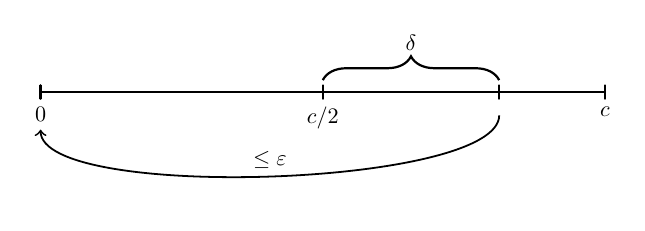
\begin{tikzpicture}[x=1.12cm, scale=0.8, every node/.append style={transform shape}]
    \draw[line width=0.2ex, line cap=round] (0,0) -- (8,0); %edit here for the axis
    \foreach \x in {0,4,6.5,8} % edit here for the vertical lines
    \draw[line width=0.2ex, line cap=round, shift={(\x,0)},color=black] (0pt,3pt) -- (0pt,-3pt);
    \foreach \x/\y/\z in {%
        0/$0$/a,
        4/${c/2}$/b,
        6.5/$$/c,
        8/$c$/d}
    \draw[line width=0.2ex, shift={(\x,0)},color=black] (0pt,0pt) -- (0pt,-3pt) node[below] (\z) {\y};

    \begin{scope}[line width=0.15ex]
        \path[->] (c) edge[out=-90, in=-90, looseness=0.4] node[above] {$\le \varepsilon$} (a);
    \end{scope}
    \draw [thick,decoration={brace,raise=1ex, amplitude=2ex},decorate] (4, 0) -- (6.5, 0) node[midway,above,yshift=3.5ex] {$\delta$};
\end{tikzpicture}

